\section{Numerical validation}\label{sec:numerics}

The replication package separates theorem-aligned simulation, deterministic rate checks, and deliberate assumption-failure experiments. The one-dimensional heat equation uses
\[
 \lambda_k=\pi^2k^2.
\]
\begin{remark}[Verification of the standing assumptions for the benchmark model]\label{rem:heat-verify}
All abstract hypotheses are fulfilled for the one-dimensional Dirichlet heat equation with $q_k\equiv1$, $u_0=0$, $\sigma_0>0$:
(i) $A_0=\partial_{xx}$ on $D=(0,1)$ with Dirichlet boundary is self-adjoint, negative, with compact resolvent, $\lambda_k=\pi^2k^2$, $e_k=\sqrt2\sin(k\pi x)$, and Weyl growth holds with $d=1$;
(ii) trace condition: $\sum_kq_k^2/\lambda_k=\pi^{-2}\sum_kk^{-2}<\infty$ (\Cref{ass:core});
(iii) pathwise Galerkin condition: $\sum_kq_k^2\lambda_k^{2(\alpha+\delta)-1}<\infty$ iff $\alpha+\delta<1/4$, as recorded after \Cref{thm:semantics};
(iv) regime (\Cref{ass:regime}): $\lambda_N\Delta_n=\pi^2N^2T/n\to0$ iff $N^2/n\to0$; the design path $n=80N^2$ holds $\lambda_N\Delta_n=\pi^2T/80\approx0.123$ \emph{constant} (as recorded in the archived design table), so the experiments probe the joint regime at a fixed small resolution while $N$ and $n$ grow --- strict theorem alignment would let $n/N^2$ diverge slowly, at higher cost and, per the reported diagnostics, no visible change; the initial-energy condition holds trivially with $u_0=0$;
(v) spectral-growth condition of the consistency proof: $N\sqrt{\lambda_N}=\pi N^2=o(\Lambda_N)$ since $\Lambda_N\sim\pi^2N^3/3$;
(vi) target class: $\widetilde\Theta\Subset(0,\infty)$, compact threshold and weight sets, and $\inf_{a,w}V_a(w)>0$ on the chosen ellipsoid, checked numerically alongside the runs.
\end{remark}

Because the LAN condition is $\lambda_N\Delta_n\to0$, a naive Cartesian grid in $(N,n)$ is not automatically theorem aligned. The main designs pair $n$ with $N^2$ so that $\lambda_N\Delta_n$ remains small.

\subsection{Mixed-rate likelihood}

The publication validation uses the paired designs
\[
 (N,n)\in\{(5,2000),(10,8000),(20,32000)\}
\]
with $1000$ replications per design. The information-standardised empirical standard deviations are within approximately $2.2\%$ of one. Drift bias and likelihood-ratio remainders contract with $N$.

\begin{table}[t]
\centering
\caption{Information-standardised estimation diagnostics.}
\begin{tabular}{rrrrr}
\toprule
$N$ & $n$ & $\mathrm{sd}(Z_\theta)$ & $\mathrm{sd}(Z_\sigma)$ & $\mathrm{bias}(\widehat\theta)$\\
\midrule
5  & 2000  & 1.0180 & 1.0062 & $3.41\times10^{-3}$\\
10 & 8000  & 1.0219 & 0.9990 & $4.5\times10^{-4}$\\
20 & 32000 & 0.9995 & 0.9955 & $-9.86\times10^{-5}$\\
\bottomrule
\end{tabular}
\label{tab:lan-num}
\end{table}

\begin{figure}[t]
\centering
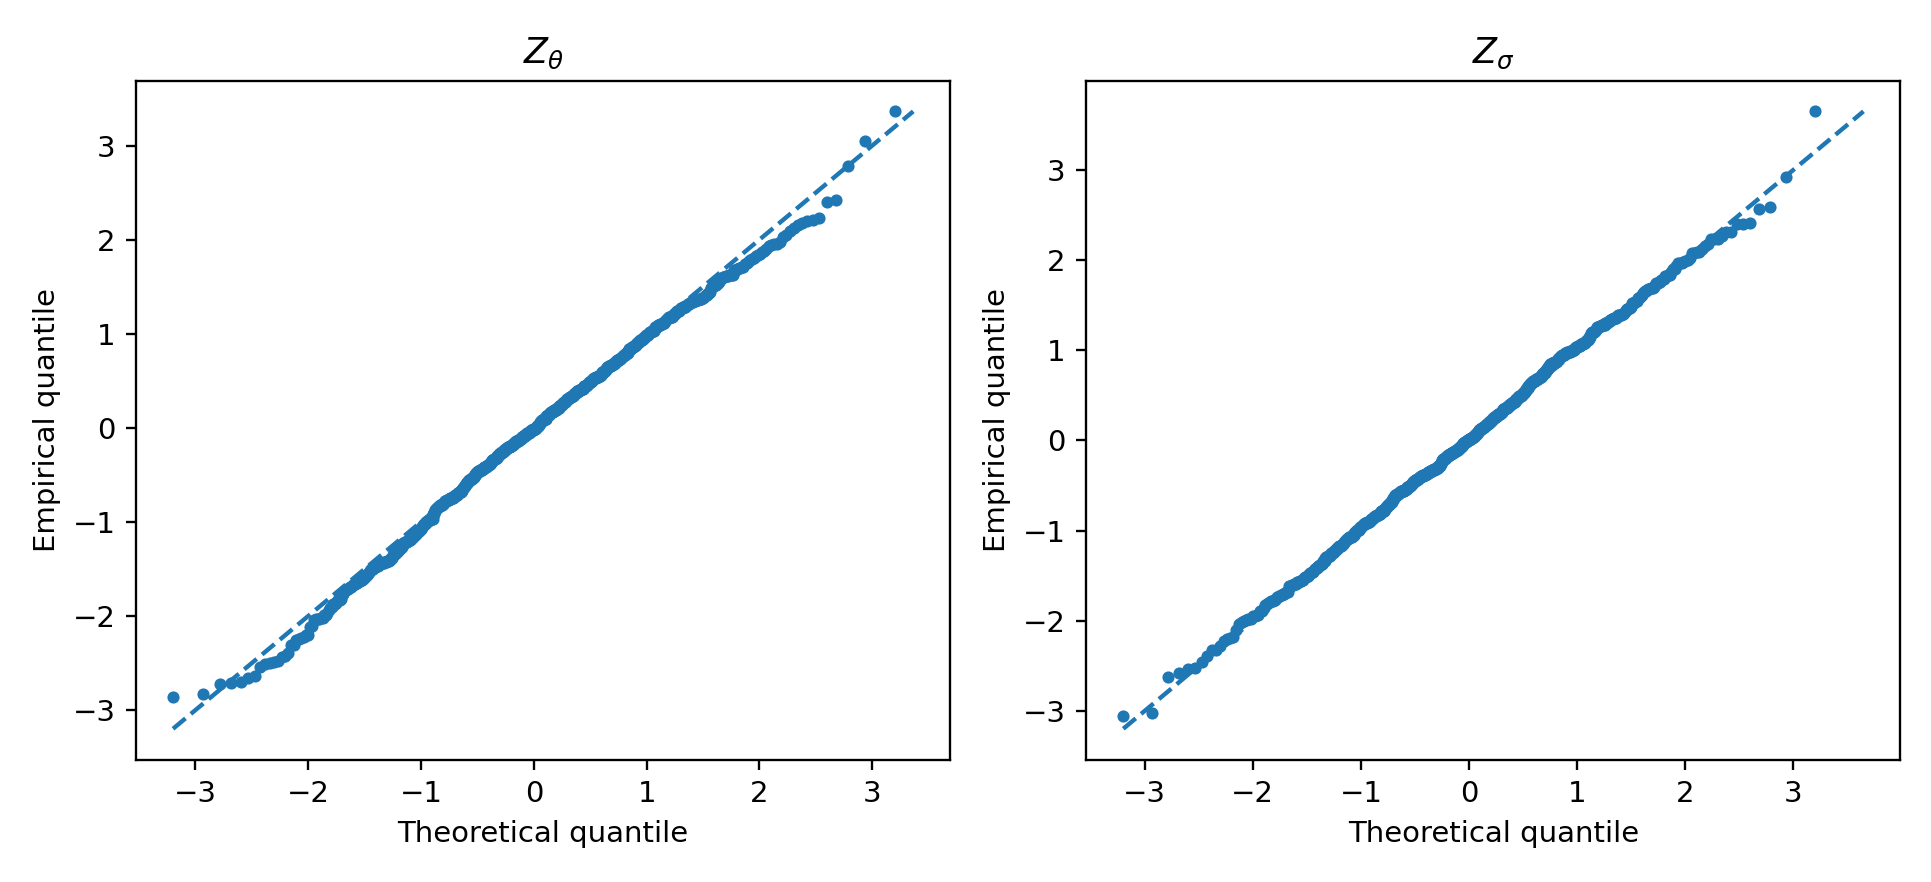
\includegraphics[width=.82\textwidth]{lan_qq_plots.png}
\caption{Normal quantile--quantile diagnostics for the standardised estimators. The visible right-skew of $Z_\theta$ at $N=5$ (skewness $0.49$, Kolmogorov--Smirnov $p=0.021$) dissipates along the design path ($p=0.42$ at $N=10$, $p=0.75$ at $N=20$), consistent with the first-order asymptotics.}
\label{fig:lan-qq}
\end{figure}

\subsection{Counterfactual process and bootstrap}

Fixed-intervention CDF sup-norm RMSE decreases from approximately $1.72\times10^{-3}$ to $2.13\times10^{-4}$. Distributional-effect sup-norm RMSE decreases from $1.64\times10^{-2}$ to $2.26\times10^{-3}$. Simultaneous coverage remains close to $0.95$ for both rate families.

\begin{table}[t]
\centering
\caption{Uniform target error and simultaneous coverage.}
\begin{tabular}{rrrrr}
\toprule
$N$ & CDF sup RMSE & Effect sup RMSE & Fast coverage & Slow coverage\\
\midrule
5  & $1.72\times10^{-3}$ & $1.64\times10^{-2}$ & 0.946 & 0.950\\
10 & $6.04\times10^{-4}$ & $6.29\times10^{-3}$ & 0.955 & 0.948\\
20 & $2.13\times10^{-4}$ & $2.26\times10^{-3}$ & 0.951 & 0.951\\
\bottomrule
\end{tabular}
\label{tab:coverage}
\end{table}

\begin{figure}[t]
\centering
\begin{subfigure}{.46\textwidth}
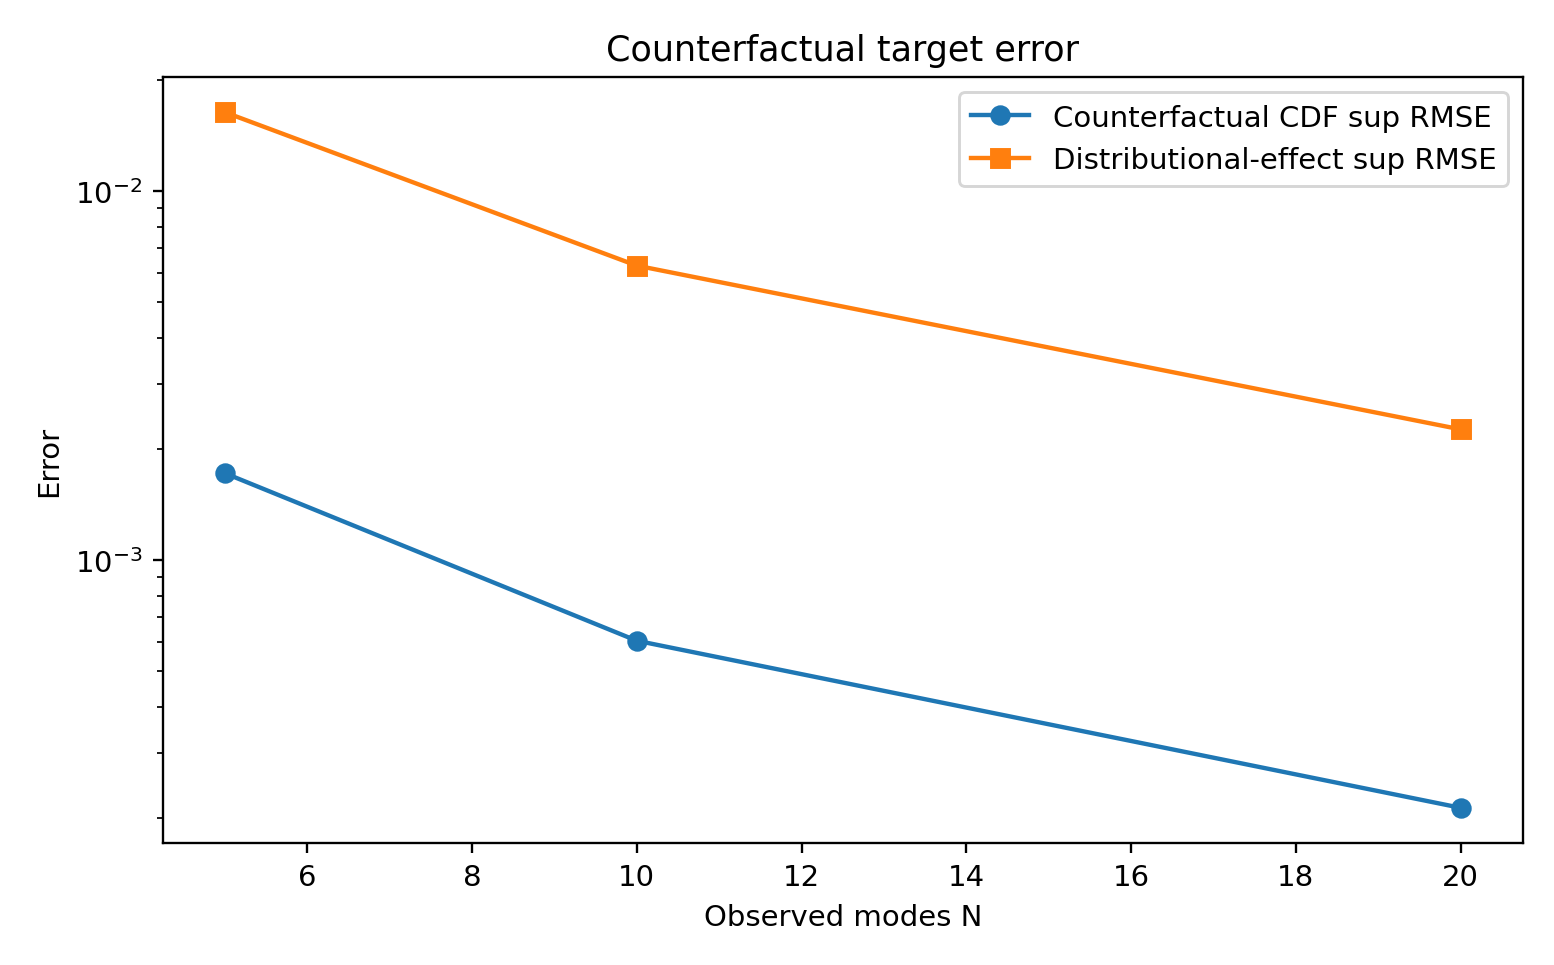
\includegraphics[width=\textwidth]{counterfactual_target_errors.png}
\caption{Uniform target errors.}
\end{subfigure}
\begin{subfigure}{.46\textwidth}
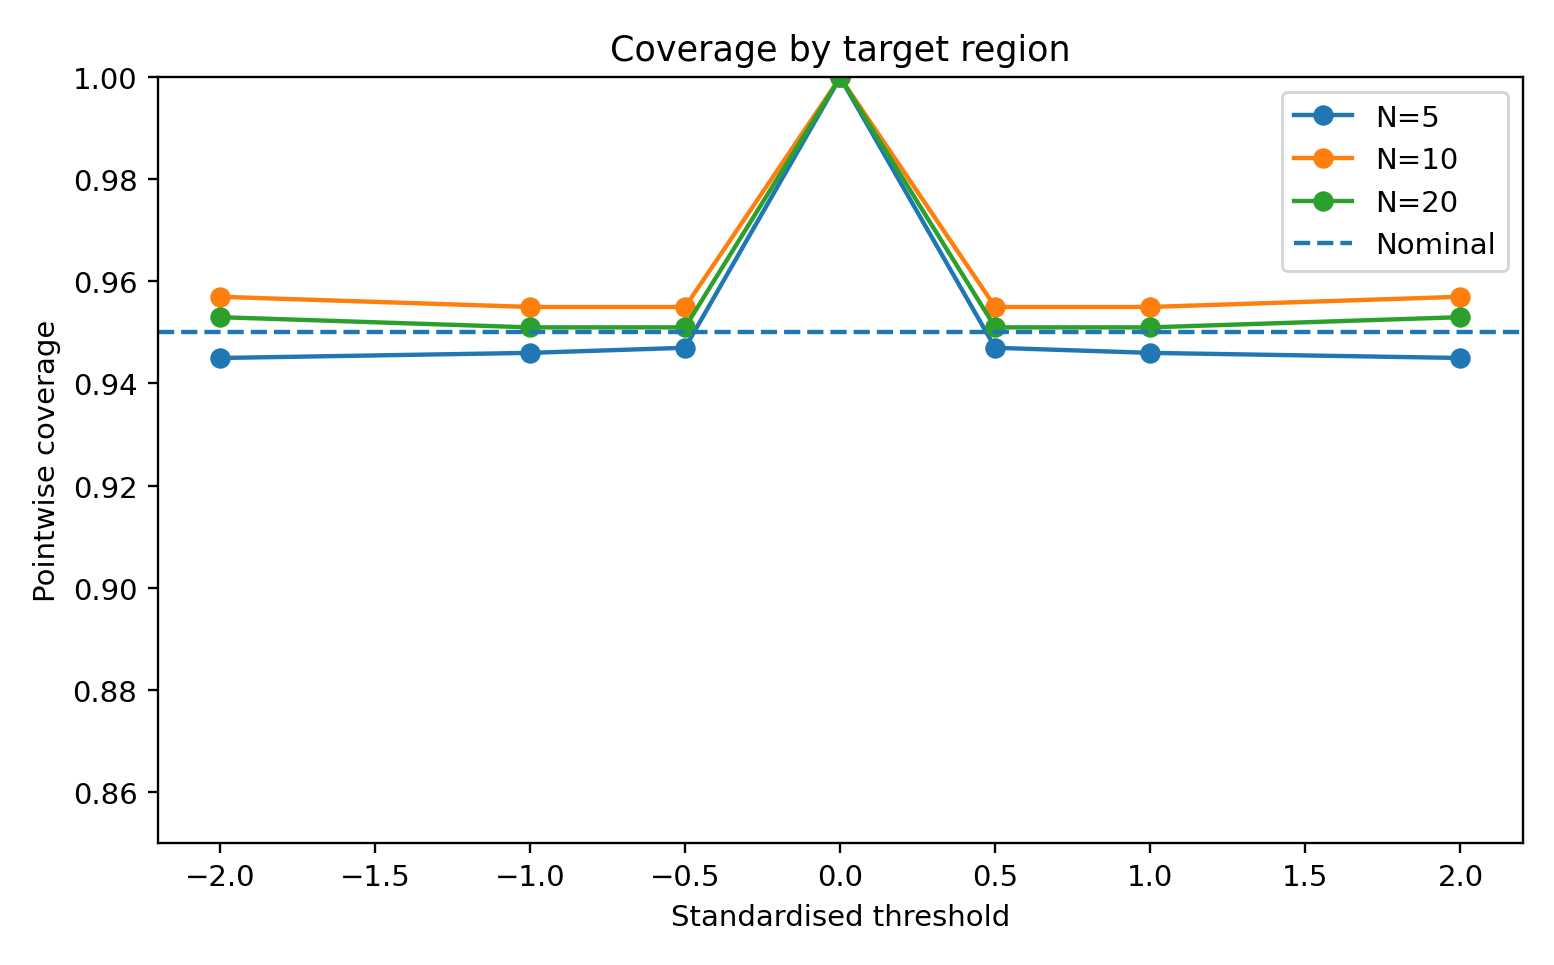
\includegraphics[width=\textwidth]{pointwise_coverage_by_threshold.png}
\caption{Coverage across thresholds.}
\end{subfigure}
\caption{Counterfactual target accuracy and coverage.}
\end{figure}

Beyond the headline coverage, the multiplier construction itself was stress-tested at $(N,n)=(10,8000)$ with $300$ replications per variant: the direct Gaussian draw, the modal-score multiplier with Gaussian weights, and the modal-score multiplier with Rademacher weights give statistically indistinguishable simultaneous coverage, and coverage is flat in the number of draws and in the threshold-grid resolution.

\begin{table}[t]
\centering
\caption{Bootstrap implementation sensitivity at $(N,n)=(10,8000)$, $300$ replications per row (Monte Carlo s.e.\ $\approx0.013$); nominal level $0.95$.}
\label{tab:boot-sens}
\begin{tabular}{llrrr}
\toprule
axis & variant & draws & fast cov. & slow cov.\\
\midrule
multiplier & direct Gaussian & 499 & 0.933 & 0.930\\
multiplier & modal Gaussian & 499 & 0.960 & 0.947\\
multiplier & modal Rademacher & 499 & 0.957 & 0.947\\
draws & direct Gaussian & 199 & 0.940 & 0.937\\
draws & direct Gaussian & 999 & 0.940 & 0.927\\
grid ($11$ pts) & direct Gaussian & 499 & 0.933 & 0.927\\
grid ($61$ pts) & direct Gaussian & 499 & 0.937 & 0.920\\
\bottomrule
\end{tabular}
\end{table}

\subsection{Approximation and sensitivity}

For the baseline spatial design, fitted log--log slopes are $-2.580$ for the mean tail, $-4.564$ for the variance tail, $-2.307$ for the strong RMS error, and $-2.580$ for the Gaussian CDF error, close to the theoretical values $-2.6,-4.6,-2.3,-2.6$. Temporal slopes lie between $0.994$ and $0.999$.

\begin{figure}[t]
\centering
\begin{subfigure}{.46\textwidth}
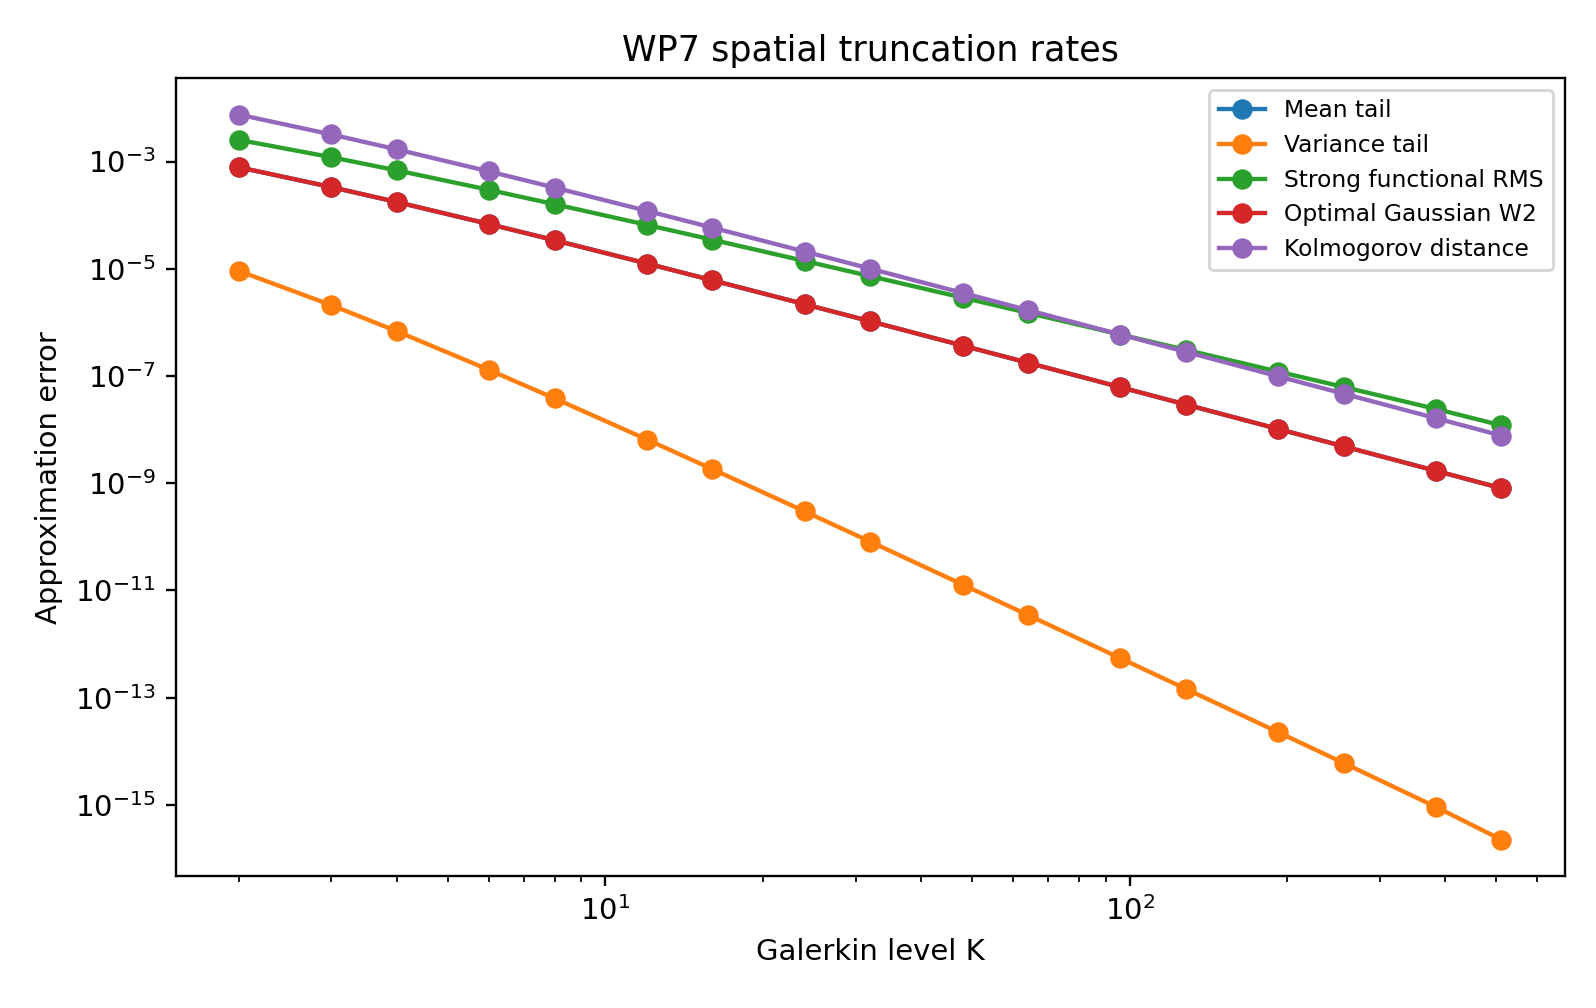
\includegraphics[width=\textwidth]{spatial_rates_baseline.png}
\caption{Galerkin rates.}
\end{subfigure}
\begin{subfigure}{.46\textwidth}
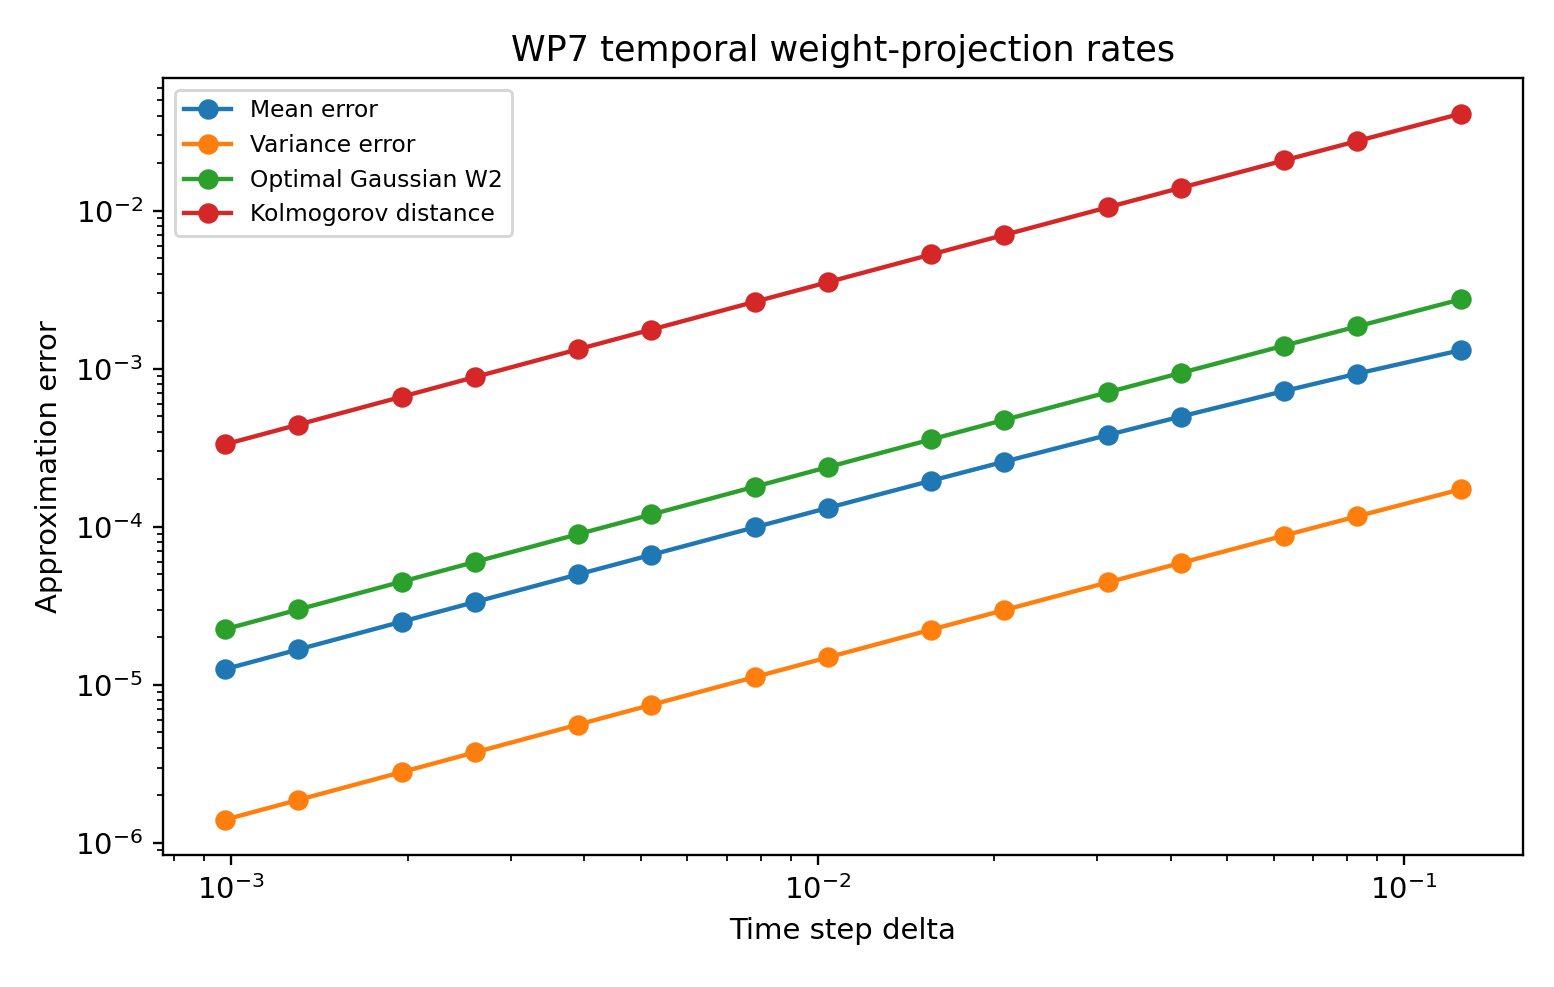
\includegraphics[width=\textwidth]{temporal_rates.png}
\caption{Temporal rates.}
\end{subfigure}
\caption{Deterministic approximation diagnostics.}
\end{figure}

For a non-commuting bounded perturbation, the central finite-difference derivative error decreases from $4.27\times10^{-6}$ at $\varepsilon=0.1$ to $1.71\times10^{-9}$ at $\varepsilon=0.002$. The CDF linearisation remainder is quadratic and the exact Gaussian $W_2$ distance remains below the derived Lipschitz envelope.

\subsection{Impossibility constructions}

The non-identification experiments are exact calculations rather than power studies. The adapted-feedback factual variance gap is zero while the post-intervention Kolmogorov distance is $0.0359$. The one-time open-loop factual variance gap is numerical zero and its post-intervention distance is $0.0984$. On a four-time grid, the factual covariance gap is $8.2\times10^{-16}$ while the post-intervention covariance gap is $0.7003$.


All tables and the headline diagnostics are regenerated by \texttt{make reproduce-publication}; the paper figures are regenerated end-to-end by the seeded validation pipeline (\texttt{make reproduce-paper}). The code records seeds, profiles, runtime, environment versions, and checksums.
